% Created 2023-05-06 Sat 15:04
\documentclass[9pt, b5paaper]{book}
\usepackage{xeCJK}
\usepackage[T1]{fontenc}
\usepackage[scaled]{beraserif}
\usepackage[scaled]{berasans}
\usepackage[scaled]{beramono}
\usepackage{graphicx}
\usepackage{xcolor}
\usepackage{multirow}
\usepackage{multicol}
\usepackage{float}
\usepackage{textcomp}
\usepackage{geometry}
\geometry{left=1.2cm,right=1.2cm,top=1.5cm,bottom=1.2cm}
\usepackage{algorithm}
\usepackage{algorithmic}
\usepackage{latexsym}
\usepackage{natbib}
\usepackage{minted}
\newminted{common-lisp}{fontsize=\footnotesize}
\usepackage[xetex,colorlinks=true,CJKbookmarks=true,linkcolor=blue,urlcolor=blue,menucolor=blue]{hyperref} 
\author{deepwaterooo}
\date{\today}
\title{plan}
\hypersetup{
  pdfkeywords={},
  pdfsubject={},
  pdfcreator={Emacs 28.2 (Org mode 8.2.7c)}}
\begin{document}

\maketitle
\tableofcontents


\chapter{Weekly Plan}
\label{sec-1}
\section{总结题型}
\label{sec-1-1}
\begin{itemize}
\item 昨天晚上两次车发动机车呜声把人从睡梦中吵醒,很过分,两次!声音的来源
是车库前一个室友的车;另一个是午夜回归的人厚重的前门开关门声,这些都
成了周五晚上他们的必使手段,只是越来越过分了。。。。。。
\item dynamic programming二刷:308 open questions, 最后几个数字相关的题写得很奔溃,第二遍终于刷完了,感觉自己比较慢知慢觉,对于比赛中的字符串和数字相关的题有种近乎死灰一样的不喜欢。。。。。。
\item 接下来的计划:觉得自己悟性不够,还需要多练习,会用接下来两三个周、一个月左右的时间(新年前)把所有剩下hard的、和medium的题做完,同时开始考虑、准备和着手安卓和unity项目,已经四个月了(从8月算起,8 9 10 11)不能再死刷题了,还是需要一些项目上的练习,再详细的计划会清晰后列出来
\item leetcode最后的几个open problem会抽时间慢慢写,但再写这些琐碎的题目兴趣不大(周赛会保持继续参加)。
\begin{itemize}
\item 昨天写这话的时候,我还没能意识到最近一段时间最近两三个周吧,自己的状态很差,主要是睡眠的问题,因为晚上休息不好,第二天的精神很差,头像顶着一团棉花昏昏头脑不够清醒,严重影响了自己的精神状态和做题。今天意识到这个问题,会从网上再多搜索一下分析一下可能的原因,并及时作调整,希望能尽快恢复过来。
\item 刷题还真是检测睡眠质量的晴雨表,冲着这一点儿,冲着到今天我才真正意识到这段时间睡眠质量是有问题的,题还得刷下去。。。一生中我从不曾像今年像这一两个月如此关注监控自己的健康与睡眠,但也都是好事,意识到问题的存在、警钟长鸣,及时调整、只有一再检测监控这些作息与生活习惯规律,才能发掘出比较高的效率与潜能。希望曾经相对比较好一些的状态能尽快调整回来(找到原因了,天气冷了,大概10号左右加了床被子太热,显著降低了睡眠质量,每天都很头痛,这两天拿走那多的一床被子,感觉好了很多。先前几个月前的7月头的时候也出现过因为门窗过于密闭而大脑缺氧一关好门窗静下来写题目就头痛过)
\end{itemize}

\item \textbf{希望这个周能抽些时间搜索一下、列一个安卓学习、复习、面试准备计划,以后的重点应该就转向按小项目来写和更新了} 这个也是实情,有很好的安卓基础,有比较强的学习意愿,只是在自己总结不够、想要边学习边做项目边总结之前,搜索一下它人是如何进阶学习准备的,想要计划出几个学习版块,计划几个小项目写出来,这个月暂时与刷题并行往前走。这几天先看一下自定义视图系列

\item 再这之后,会写一些Android Project,同时大量发简历、找工作,并每天抽部分时间(可能几个小时吧)继续总结和刷完剩下不感兴趣、或觉得不值一写的几个leetcode open problems.

\item 但不管接下来自己的项目是集中在安桌上,还是向unity game偏,leetcode和codeforce的周赛、比赛等都还是会尽量参加、在精神状态允许下,争取把题目都写出来

\item 完成打基础的部分: hashing, hashmap, string, two pointer, sliding window,这些基础部分的题目,希望扫完
\item 如果某天头脑比较清醒、精力比较好的时候,会试图去慢速解决自己平时困难的地方:动态规划/ hashmap/hashing中数数组的个数,不常用的算法等

\item 数组相关的 segemnt tree, binary index tree等的基础,希望能够理解得再彻底一些,到能活学活用的程度
\item Deque双端队列O(n)解法的概念在建立,还需要很多的练习和熟悉
\item 最讨厌扫描线和数字相关的,几个双数怎么也数不清楚 heap等。。。。。。这个周扫几个出去

\item 如果说以前是迷迷糊糊刷题求AC,现在基本的概念在建立,希望从以前代码和题目的算法效率向代码优化中等偏优,寻求高效、最优解法的提升
\item bit manipulation, bitmasks基础知识基本掌握,还剩几道难题take my time慢慢解(感觉现在对bit操作,相对自信得心应手得多了!)
\item union find 的几个题,基本算是基本扫完吧,剩下的几下慢慢写。。。。。。

\item 经过一段时间的饮食调理,现在右耳单耳电磁波一样的叫声已经小了很多,希望通过再多一段时间的饮食调理它会自动消失掉。前天和昨天连续两天晚上都没能消息好(前天晚上可能是因为在它们炒作的枪口上写出了自己一直以来的愿望吧,昨天一天、到晚上明明已经很累了,晚上还出去稍微运动了一下希望晚上能早点儿入睡能休息好,却偏偏还是没能安时入眠),直接导致今天早上起床稍微有点儿困难,我比较喜欢现在这个自9月来养成的早上6点起床的极少失眠的作息(这两三个月来也没再喝咖啡),希望赶快把作息再次调整恢复正常(现在还不想换成浪费早上时候,午休90分钟深睡眠的作息)。
\end{itemize}

\section{比赛}
\label{sec-1-2}
\begin{itemize}
\item 会尽量多参加一些比赛,比赛时的效率还是相对好一点儿,所以leetcode上以后每周一次、每半月一次,以及以后codeforces上的比赛,希望都能够尽量地多参加一些。
\item codeforces 的刷题界面还不是很熟悉,对于暴内存之类的问题尚没有思考,需要再熟悉一下,希望也能尽量多参加他们家的比赛,希望参加他们家的比赛能够自己写得出答案

\item 今天的两场,早上的题目不难,但比较坑人,考得偏,越是怕数个数什么的,越是几个题三四个题都故意挑你的刺(我觉得早上他们是想要找茬来着。。。想抓我再冷嘲热讽一番,可惜抓不住了。。)。晚上的前三个题都简单,半个小时全做出来了,可是最后一题读不懂题目,不知道它在说什么,上次的union find 第四题难题做出来了,今天说的是同样考点却没能认出来。
\item 简单的题慢慢地已经不再是重点,希望以后能尽量地把难题做出来,像做今天早上比赛的最后一题一样,因为晚上休息不好(鬼窝里的恶鬼惯性地周五晚上都会故意洗手间弄很久故意吵人,像今天两场比赛的也会在我午休等休息时间故意吵你休息,今天中午我平时做饭时间有人做了大半个小时,我等不及没办法自己泡了袋面吃,下午4:30一杯热水喝下去,感觉人都快饿虚脱了。。。),早上起来拿鸡蛋掉到了地上,走路撞到桌子角,但脑袋再昏,写早上的那个不算难的数数的第四题,还是写得思路极为清晰,像蓝天白云一样清澈见底。其它偏一点儿、脑袋急转弯一样的题,希望以后也能慢慢学会处理。
\item 早上抓人没抓着,晚上应该是给糖吃吧,可惜最后一题读不懂题目,其它三题好简单
\item 每周周六周日节假日对我来说是最难过的,因为恶鬼都在家,他们有白天休息时间,晚上你要休息时他们有的是办法故意扰你休息,周一到周五反而相对较好,毕竟他们还得出去工作
\end{itemize}

\chapter{数据规模与算法}
\label{sec-2}
\begin{center}
\begin{tabular}{rl}
\hline
Input Size & Complexity\\
\hline
50000 & O(n)\\
20000 & O(n logn)\\
\hline
1000 & O(n \^{} 2)\\
30 & O(n \^{} 4)\\
16 (20) & O(2 \^{} n)\\
\hline
\end{tabular}
\end{center}


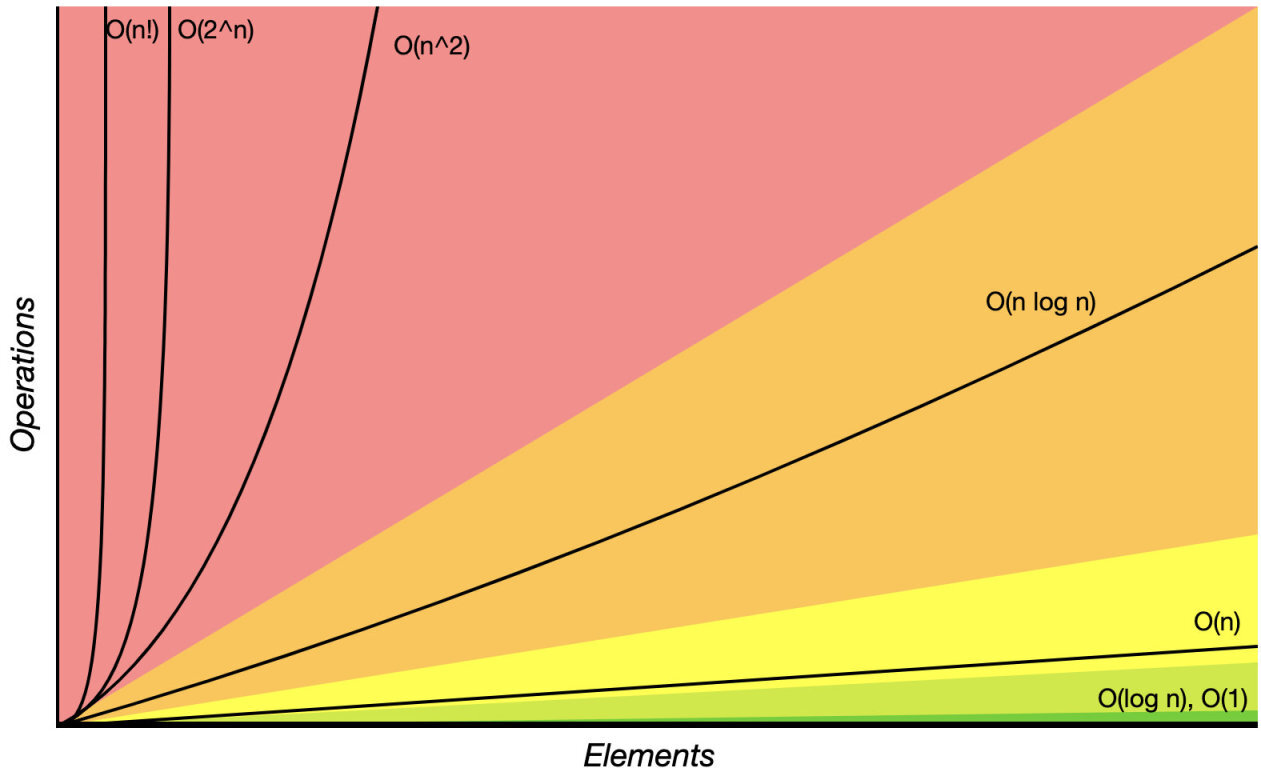
\includegraphics[width=.9\linewidth]{./pic/bigo.jpeg}

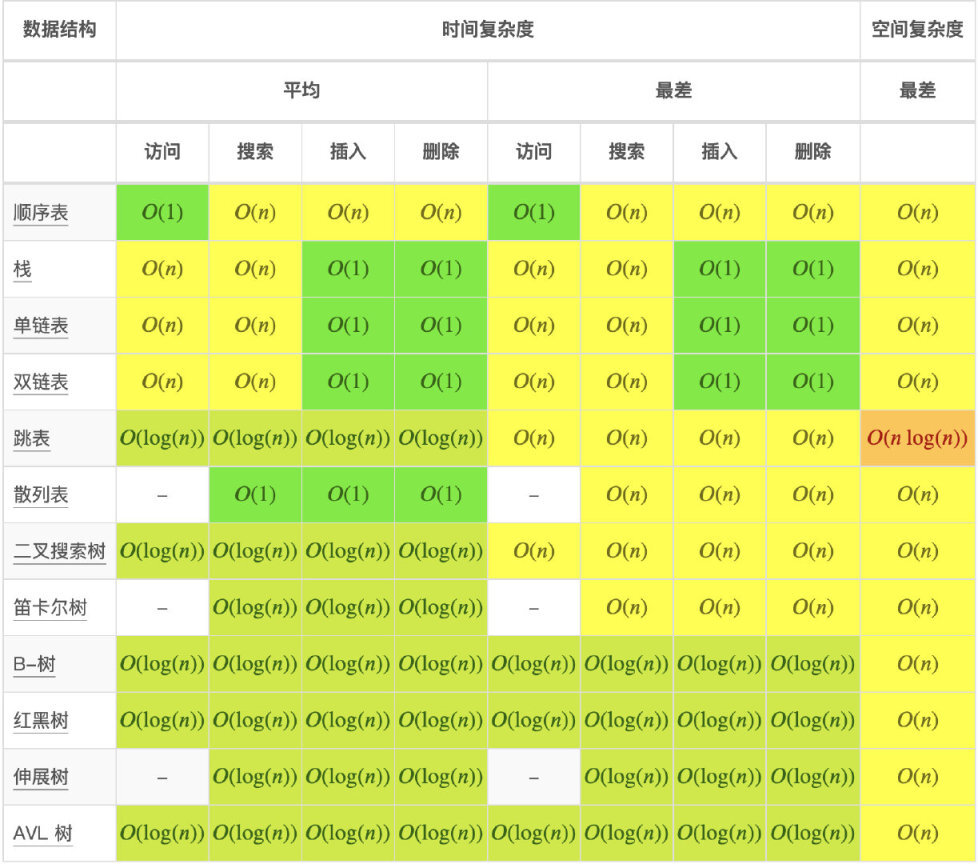
\includegraphics[width=.9\linewidth]{./pic/bigo2.jpeg}

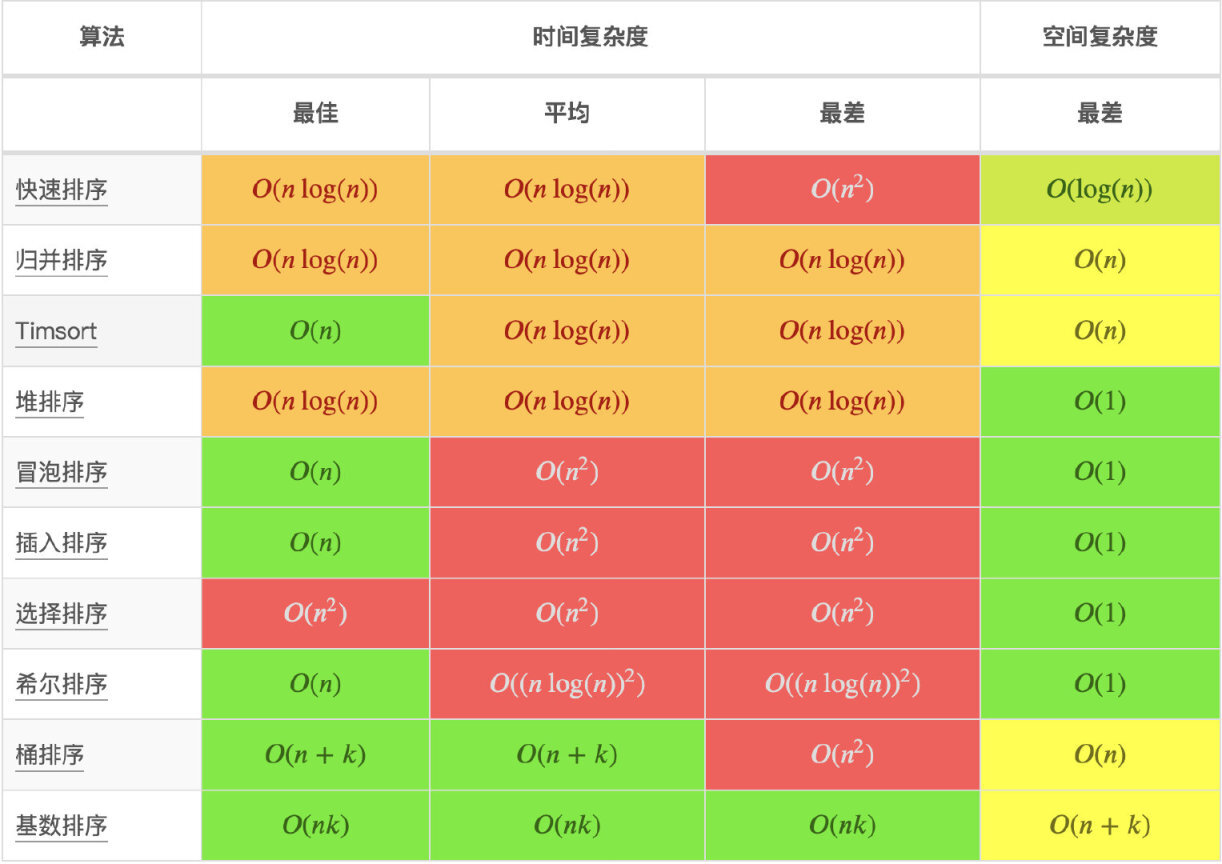
\includegraphics[width=.9\linewidth]{./pic/bigo3.jpeg}

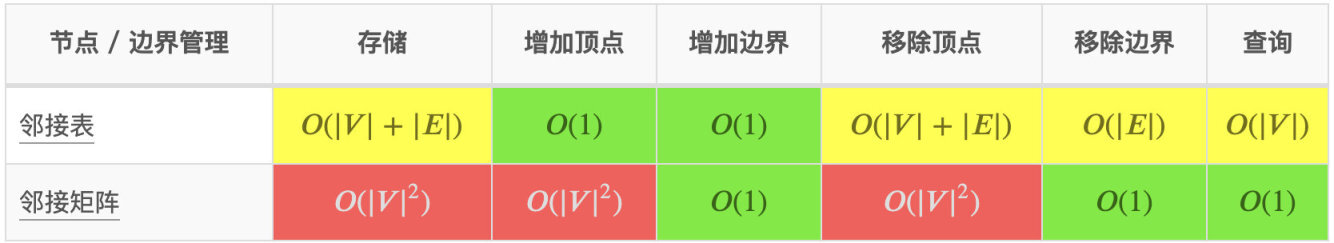
\includegraphics[width=.9\linewidth]{./pic/bigo4.jpeg}

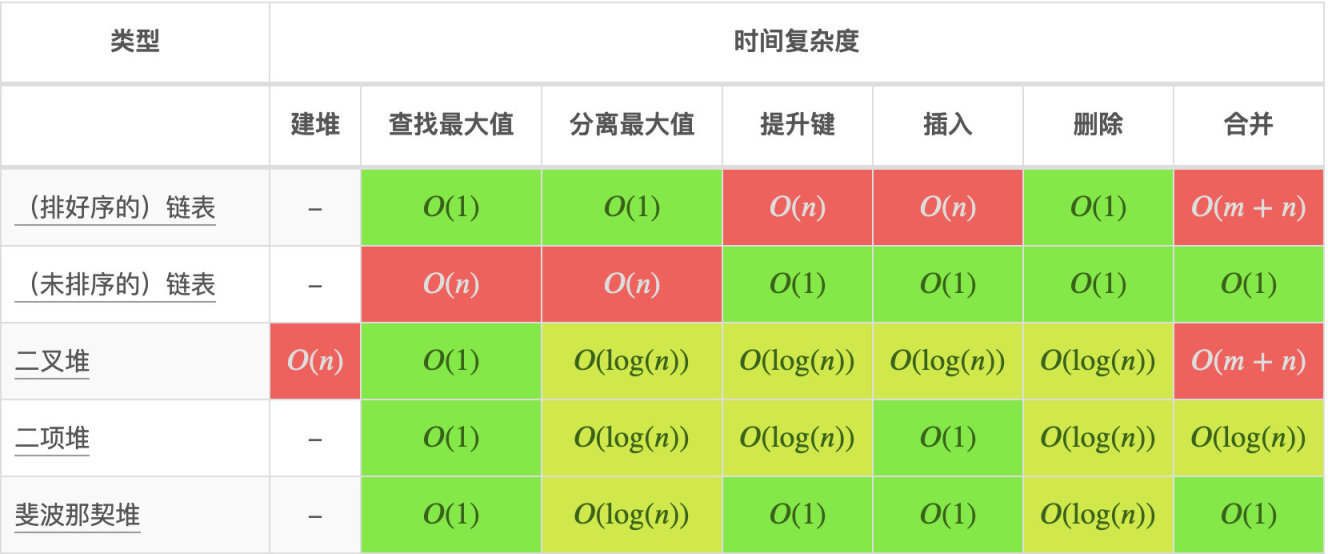
\includegraphics[width=.9\linewidth]{./pic/bigo5.jpeg}
% Emacs 28.2 (Org mode 8.2.7c)
\end{document}